\documentclass[11pt,a4paper]{article}
\usepackage[margin=1.8cm]{geometry}
\usepackage{amsmath,amssymb}
\usepackage{booktabs}
\usepackage{parskip}
\usepackage{tikz}
\setlength{\parskip}{6pt}
\setlength{\textfloatsep}{8pt}
\setlength{\intextsep}{8pt}
\usepackage[font=small, skip=4pt]{caption}

\begin{document}

\begin{center}
{\large Entanglement of a 20-qubit GHZ state on MIMIQ}\\[4pt]
Khuram Shahzad, October 2026
\end{center}

We prepared $|\mathrm{GHZ}\rangle = (|0\cdots0\rangle + |1\cdots1\rangle)/\sqrt{2}$ on
$N = 4$ to $20$ qubits (Fig.~\ref{fig:circuit}). Cut measures: MIMIQ cloud, MPS simulator
(the local MPS simulator had no free licence seat); everything else on the laptop.
Clusters: $\rho = 2^{-k}\sum_P \langle P\rangle P$ from Pauli expectation values (Exaqt),
entanglement from the thesis GCG code.

\begin{figure}[h!]
\centering
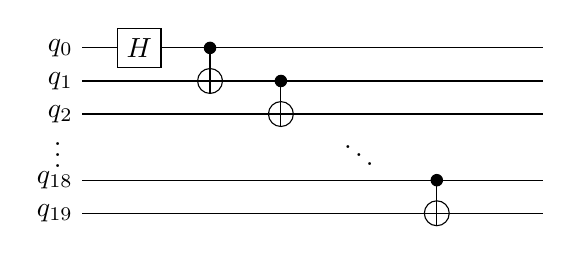
\begin{tikzpicture}[x=0.9cm, y=0.42cm,
    ctrl/.style={circle, fill, inner sep=1.6pt},
    targ/.style={circle, draw, inner sep=0pt, minimum size=9pt, path picture={
        \draw (path picture bounding box.north) -- (path picture bounding box.south)
              (path picture bounding box.west)  -- (path picture bounding box.east);}}]
  % wires: q0, q1, q2 on top, q18, q19 at the bottom (rows 0..-1..-2 and -4, -5)
  \foreach \y/\name in {0/q_0, -1/q_1, -2/q_2, -4/q_{18}, -5/q_{19}} {
    \draw (0, \y) -- (6.5, \y);
    \node[left] at (0, \y) {$\name$};
  }
  \node at (-0.35, -3) {$\vdots$};
  % H on q0
  \node[draw, fill=white, minimum size=0.5cm] at (0.8, 0) {$H$};
  % CNOT q0 -> q1
  \draw (1.8, 0) -- (1.8, -1);  \node[ctrl] at (1.8, 0) {};  \node[targ] at (1.8, -1) {};
  % CNOT q1 -> q2
  \draw (2.8, -1) -- (2.8, -2); \node[ctrl] at (2.8, -1) {}; \node[targ] at (2.8, -2) {};
  % the chain continues
  \node at (3.9, -3) {$\ddots$};
  % CNOT q18 -> q19
  \draw (5.0, -4) -- (5.0, -5); \node[ctrl] at (5.0, -4) {}; \node[targ] at (5.0, -5) {};
\end{tikzpicture}
\caption{Circuit preparing the GHZ state on a chain of $N$ qubits.}
\label{fig:circuit}
\end{figure}

For a cut at qubit $k$ ($A = \{0,\dots,k-1\}$, $B$ the rest), the two parts share one
maximally entangled bit, $S = \log_2 r = 1$, for $N = 6, 8, 10$ and $20$ alike
(Table~\ref{tab:cuts}).

\begin{table}[h!]
\centering
\small
\begin{tabular}{cccc}
  \toprule
  cut $k$ & entropy $S(\rho_A)$ (bits) & Schmidt rank & bond dimension \\
  \midrule
  0 ($A$ empty) & 0 & 1 & 1 \\
  1 to $N-1$    & 1 & 2 & 2 \\
  \bottomrule
\end{tabular}
\caption{Bipartite measures between $A$ = qubits $0,\dots,k-1$ and the rest of the chain (MIMIQ cloud, MPS); identical for $N = 6, 8, 10, 20$.}
\label{tab:cuts}
\end{table}

Every cluster is the classical mixture
$(|0\cdots0\rangle\langle0\cdots0| + |1\cdots1\rangle\langle1\cdots1|)/2$: no entanglement,
for neighbouring and for distant qubits (Table~\ref{tab:clusters}).

\begin{table}[h!]
\centering
\small
\begin{tabular}{lcccc}
  \toprule
  qubits & Pauli strings & purity & measure & value \\
  \midrule
  0, 1           & 15  & 0.5 & bipartite (0 vs 1)         & 0 \\
  0, 1, 2        & 63  & 0.5 & $\mathcal{C}_{\rm GME}$    & 0 \\
  0, 1, 2, 3     & 255 & 0.5 & $\mathcal{C}_{\rm GME}$    & 0 \\
  0, 10, 19      & 63  & 0.5 & $\mathcal{C}_{\rm GME}$    & 0 \\
  \bottomrule
\end{tabular}
\caption{Entanglement inside clusters of the 20-qubit GHZ state, all other qubits
ignored (traced out); Pauli expectation values (Exaqt), GCG convex roof.}
\label{tab:clusters}
\end{table}

For the whole state the GME concurrence is 1 at every size (Table~\ref{tab:full}). Up to
$N = 8$ it is obtained from measurements only, with $\rho$ rebuilt from all $4^N-1$ Pauli
strings, and it agrees with the value from the state vector. The number of strings grows as
$4^N$, so beyond $N \approx 8$ only the state-vector value is shown.

\begin{table}[h!]
\centering
\small
\begin{tabular}{rrcc}
  \toprule
  $N$ & Pauli strings & $\mathcal{C}_{\rm GME}$ from measurements & $\mathcal{C}_{\rm GME}$ from state vector \\
  \midrule
   4 &           255 & 1.000000 & 1.000000 \\
   6 &         4\,095 & 1.000000 & 1.000000 \\
   8 &        65\,535 & 1.000000 & 1.000000 \\
  10 &     1\,048\,575 & --       & 1.000000 \\
  16 & $4.3\times10^{9}$  & --  & 1.000000 \\
  18 & $6.9\times10^{10}$ & --  & 1.000000 \\
  \bottomrule
\end{tabular}
\caption{GME concurrence of the full GHZ state (pure-state formula, all $2^{N-1}-1$
bipartitions). State-vector values are from the simulator memory, not from measurements.}
\label{tab:full}
\end{table}

GHZ entanglement is fully collective: maximal across every cut, absent in every
smaller group. For large $N$ it cannot be measured through the $n$BRDMs; entanglement
witnesses or spin inequalities are the practical route (to discuss with QPerfect).

\end{document}
